\part{Binary notation}
\frame{\partpage}

\begin{frame}
	\centering
	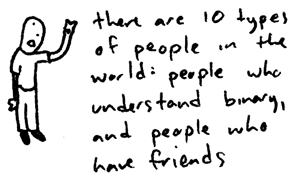
\includegraphics[width=0.7\textwidth]{10-types-of-people}
	\par\vspace{2ex}\par
	{\tiny Image credit: \url{http://www.toothpastefordinner.com}}
\end{frame}



\begin{frame}{How we write numbers}
	\begin{itemize}
		\pause\item We write numbers in \textbf{base~10}
		\pause\item We have 10 \textbf{digits}: $0, 1, 2, \dots, 8, 9$
		\pause\item When we write $6397$, we mean:
			\begin{itemize}
				\pause\item Six thousand, three hundred and ninety seven
				\pause\item (Six thousands) and (three hundreds) and (nine tens) and (seven)
				\pause\item $(6 \times 1000) + (3 \times 100) + (9 \times 10) + (7)$
				\pause\item $\left(6 \times 10^3\right)
				+ \left(3 \times 10^2\right)
				+ \left(9 \times 10^1\right)
				+ \left(7 \times 10^0\right)$
			\end{itemize}
	\end{itemize}
\end{frame}

\begin{frame}{Binary}
	\begin{itemize}
		\pause\item Binary notation works the same, but is \textbf{base~2} instead of \textbf{base~10}
		\pause\item We have 2 \textbf{digits}: $0, 1$
		\pause\item When we write $10001011$ in binary, we mean: \par\pause
			$\phantom{+} \left(1 \times 2^7\right) + 
			\left(0 \times 2^6\right) + 
			\left(0 \times 2^5\right) + 
			\left(0 \times 2^4\right)$ \par
			$+ \left(1 \times 2^3\right) + 
			\left(0 \times 2^2\right) + 
			\left(1 \times 2^1\right) + 
			\left(1 \times 2^0\right)$ \par\pause
			$= 2^7 + 2^3 + 2^1 + 2^0$ \par\pause
			$= 128 + 8 + 2 + 1 \text{ (base 10)}$ \par\pause
			$= 139 \text{ (base 10)}$
	\end{itemize}
\end{frame}

\begin{frame}{Bits, bytes and words}
	\begin{itemize}
		\pause\item A \textbf{bit} is a \uline{b}inary dig\uline{it}
			\begin{itemize}
				\pause\item Can store a 0 or 1 (i.e.\ a boolean value)
			\end{itemize}
		\pause\item A \textbf{byte} is 8 \textbf{bits}
			\begin{itemize}
				\pause\item Can store a number between 0 and 255 in binary
			\end{itemize}
		\pause\item A \textbf{word} is the number of bits that the CPU works with at once
			\begin{itemize}
				\pause\item 32-bit CPU: 32 bits = 1 word
				\pause\item 64-bit CPU: 64 bits = 1 word
			\end{itemize}
		\pause\item An $n$-bit word can store a number between 0 and $2^{n} - 1$
			\begin{itemize}
				\pause\item $2^{16}-1 = 65,535$
				\pause\item $2^{32}-1 = 4,294,967,295$
				\pause\item $2^{64}-1 = 18,446,744,073,709,551,615$
			\end{itemize}
	\end{itemize}
\end{frame}

